\section{Related Works}

\begin{frame}{Taxonomy of Related Works}
    \begin{figure}
        \centering
        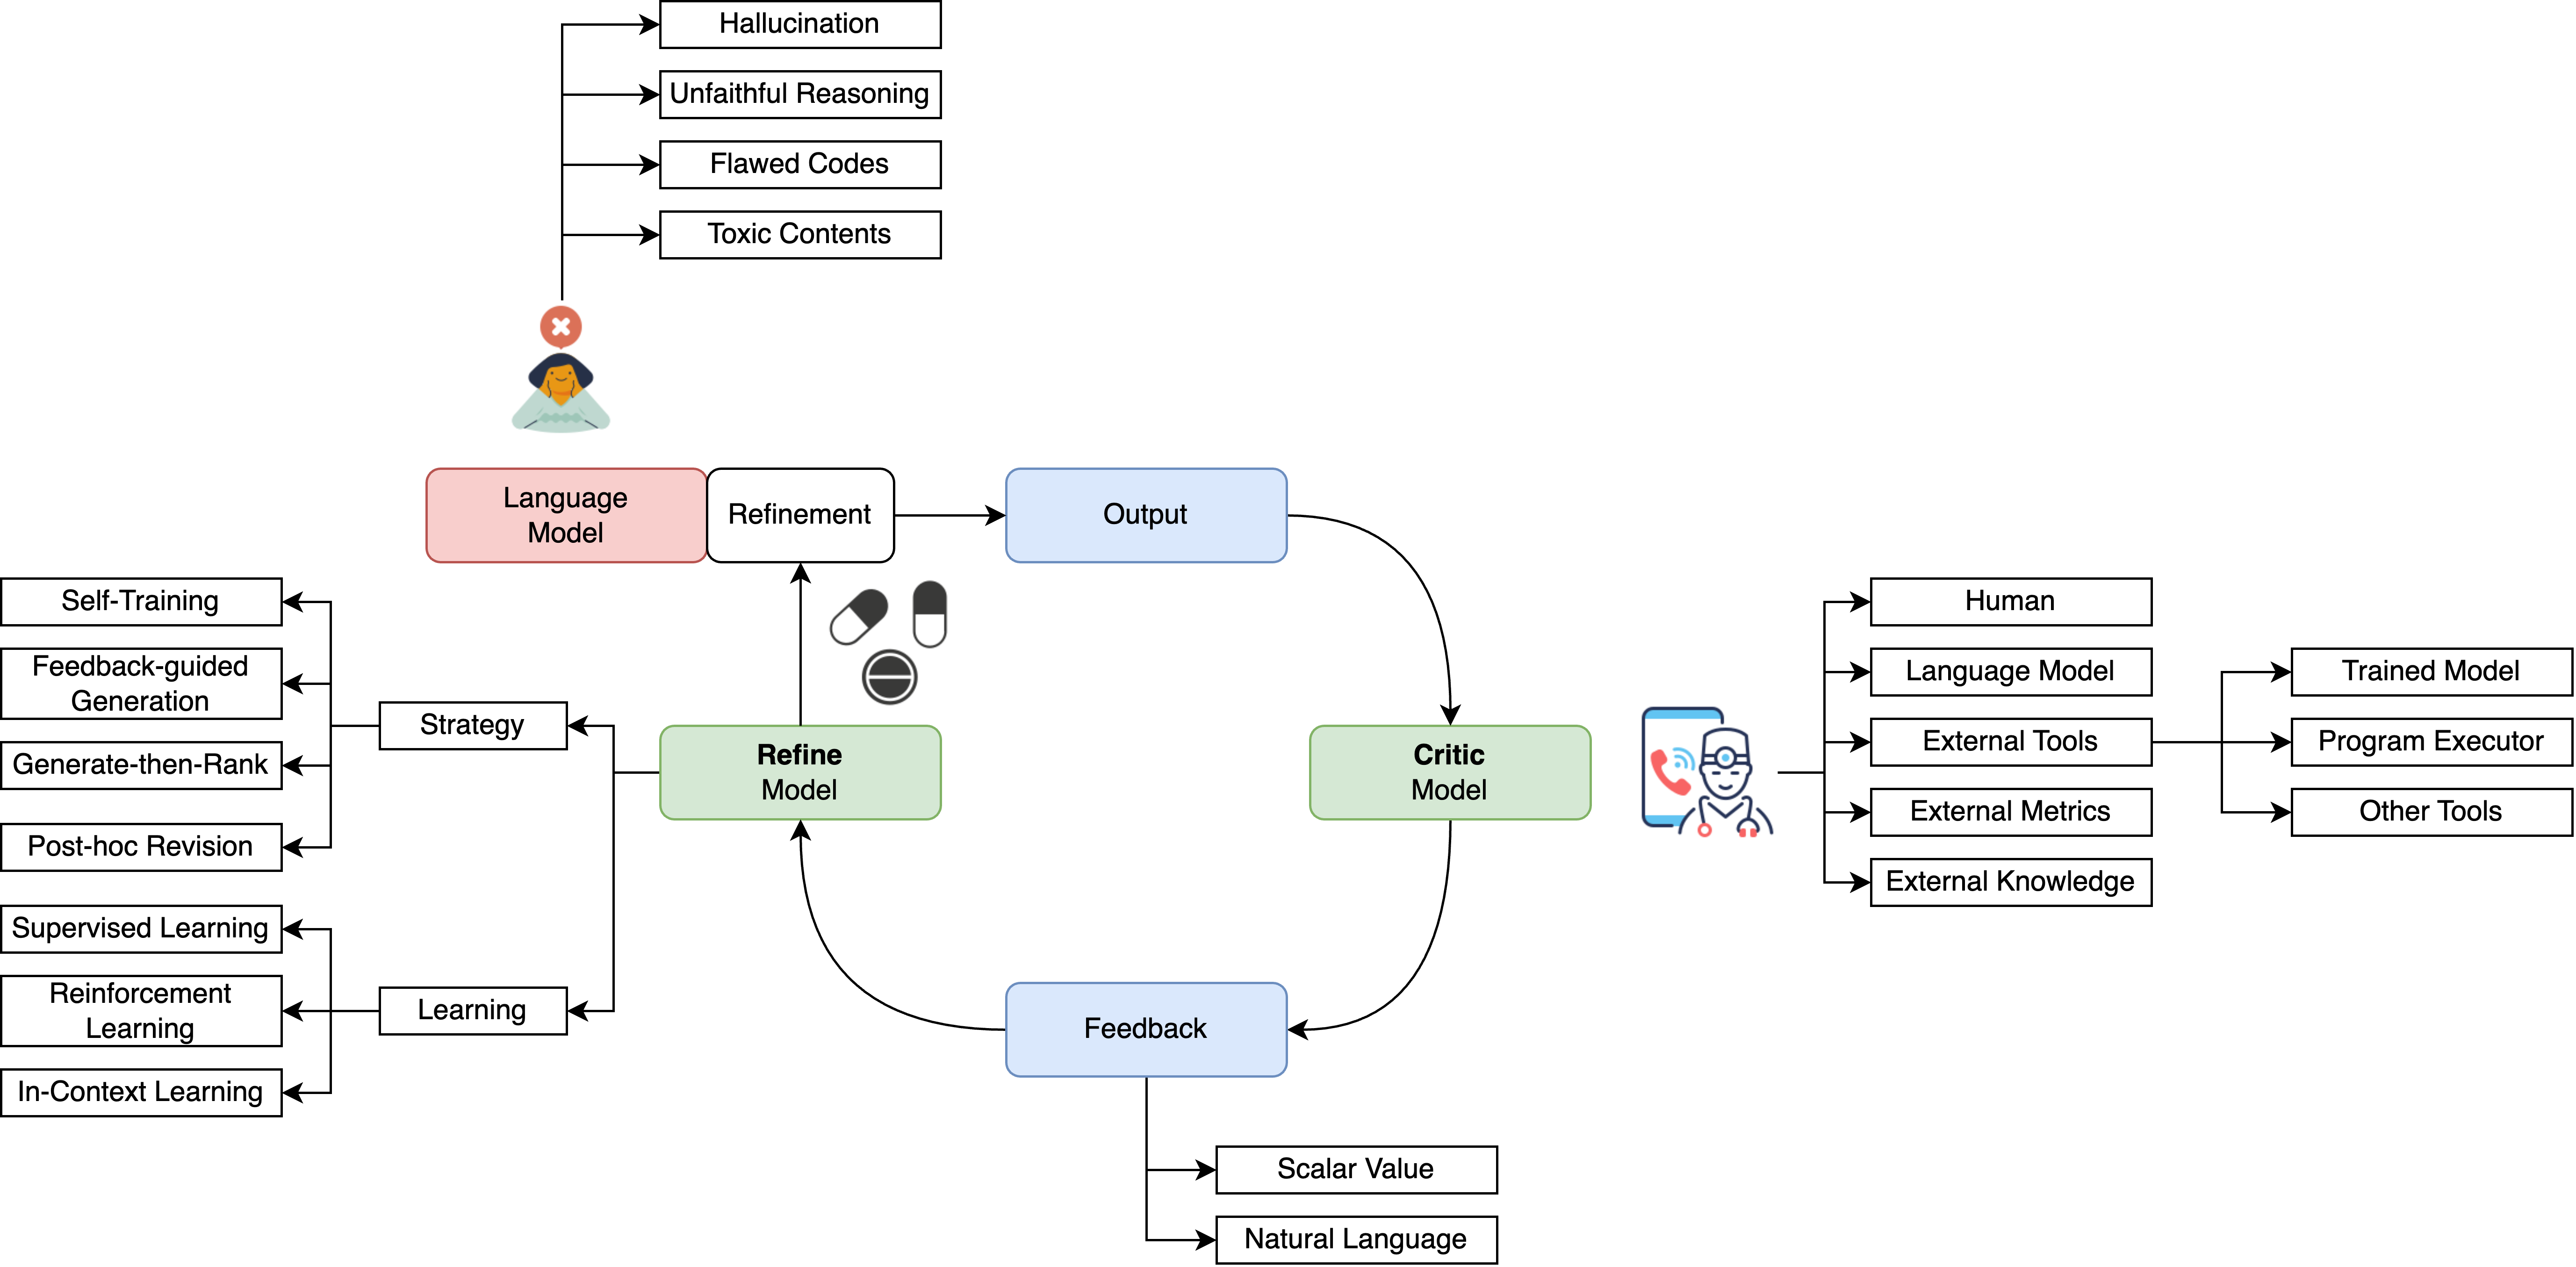
\includegraphics[width=1\textwidth]{img/taxonomy}
        \captionsetup{font=small,labelformat=empty}
        \caption{Taxonomy of works on self-correcting LLMs.}\label{fig:taxonomy}
    \end{figure}
\end{frame}

\begin{frame}{Problems of LLMs}
    \begin{columns}[T]
        \begin{column}{0.70\textwidth}
            The works aimed at correcting LLMs can be classified according to the issues they tackle:
            \begin{enumerate}
                \item Hallucination: plausible-sounding but false information~\cite{gao2023rarr, zhang2023language}.

                \item Unfaithful Reasoning: derived conclusion does not follow the previously generated reasoning chain~\cite{he2022rethinking, pan2023logiclm}.

                \item Toxic Contents: content that is toxic, biased, or harmful due to biases present in the training datas~\cite{lu2022quark, gou2023critic}.

                \item Flawed Codes: flawed or incorrect code generation~\cite{chen2023teaching, olausson2023selfrepair}.
            \end{enumerate}
        \end{column}
        \begin{column}{0.30\textwidth}
            \begin{figure}[!htb]
                \centering
                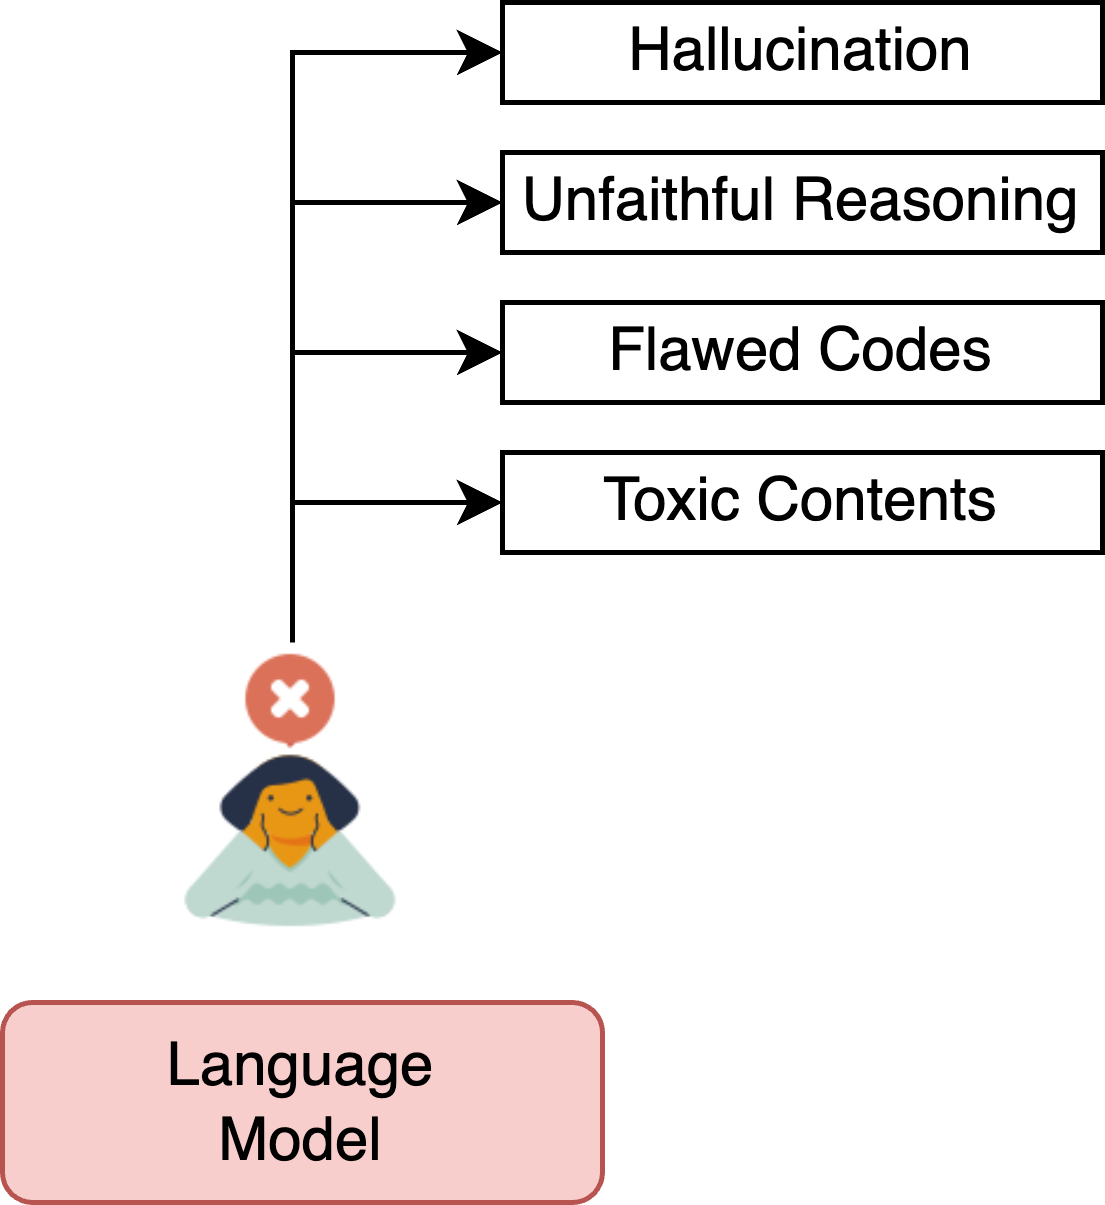
\includegraphics[width=1\textwidth]{img/language_model}
                \captionsetup{font=small,labelformat=empty}
                \caption{Problems of LLMs.}
            \end{figure}
        \end{column}
    \end{columns}
\end{frame}

\begin{frame}{Critic Model}
    \begin{columns}[T]
        \begin{column}{0.55\textwidth}
            Source of feedback:
            \begin{enumerate}
                \item Self-Feedback: the model itself generates feedback~\cite{weng2023large}.

                \item External Feedback: the model receives feedback from an external source (e.g., human, program executor and external knowledge)~\cite{gou2023critic}.
            \end{enumerate}

            Format of feedback:
            \begin{enumerate}
                \item Scalar Value: metrics based on pre-defined tests~\cite{weng2023large}.

                \item Natural Language: provides richer information than scalar value feedback~\cite{chen2023teaching}.
            \end{enumerate}
        \end{column}
        \begin{column}{0.45\textwidth}
            \begin{figure}[!htb]
                \centering
                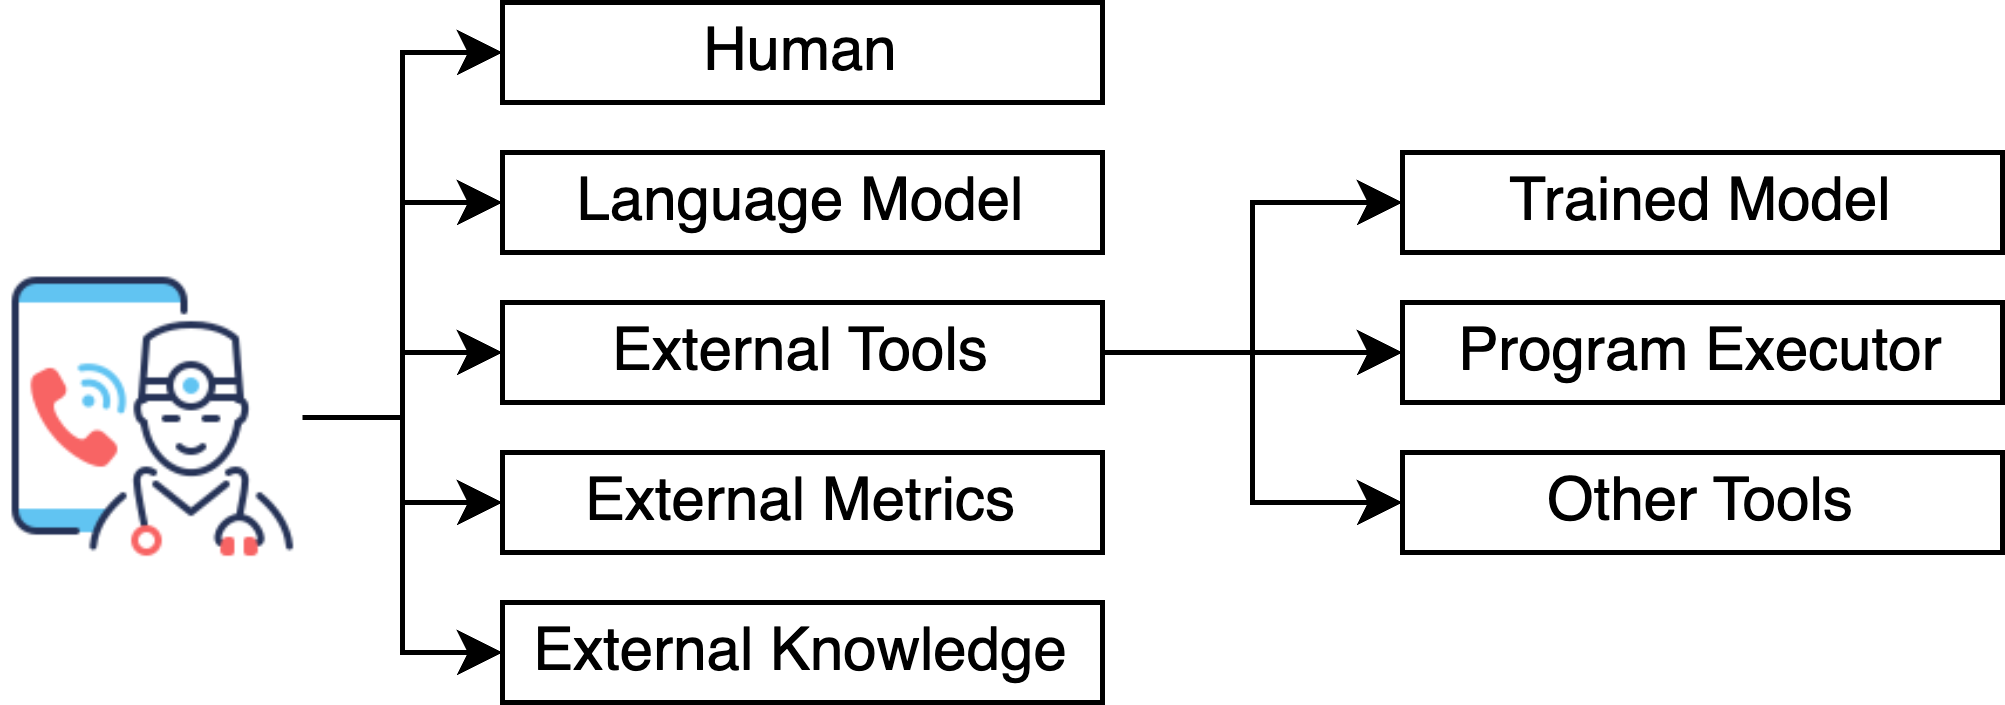
\includegraphics[width=1\textwidth]{img/critic_model}
                \captionsetup{font=small,labelformat=empty}
                \caption{Critic Model.}
            \end{figure}
        \end{column}
    \end{columns}
\end{frame}

\begin{frame}{Refine Model}
    The Refine Model is the most active area of research in the field. Existing works can be classified based on the following key questions:
    \begin{enumerate}
        \item Need to update the LLMs? \textbf{Yes}: Self-Training~\cite{huang2022large}, Supervised Learning~\cite{bai2022training}, Reinforcement Learning~\cite{dubois2024alpacafarm}, In-Context Learning~\cite{dong2022survey}.

        \item When to refine: generation-time or post-hoc?
              \begin{itemize}
                  \item Generation-time: Generate-then-Rank~\cite{cobbe2021training}, Feedback-Guided Generation~\cite{yao2023tree}.
                  \item Post-hoc: Models/Tools as Feedback~\cite{zhang2023selfedit}, Multi-Agent Debate~\cite{du2023improving}.
              \end{itemize}
    \end{enumerate}
\end{frame}

\begin{frame}{Obstacles and Prospects}
    \begin{enumerate}
        \item Obstacle: Predominantly, existing LLMs, like OpenAI's GPT-4, are proprietary. Alternatively, they may possess an impractically vast number of parameters for training within the confines of this study, as seen in the 70-billion parameter LLaMa model.

        \item Prospect: A number of notable studies have been conducted on the utilization of self-correcting LLMs in autonomous code correction. Examples include Google Deepmind's SelfDebug~\cite{chen2023teaching} and Shanghai Jiao Tong University's SelfEvolve~\cite{jiang2023selfevolve}.
    \end{enumerate}
\end{frame}

\begin{frame}{Research Direction}
    \begin{figure}[!htb]
        \centering
        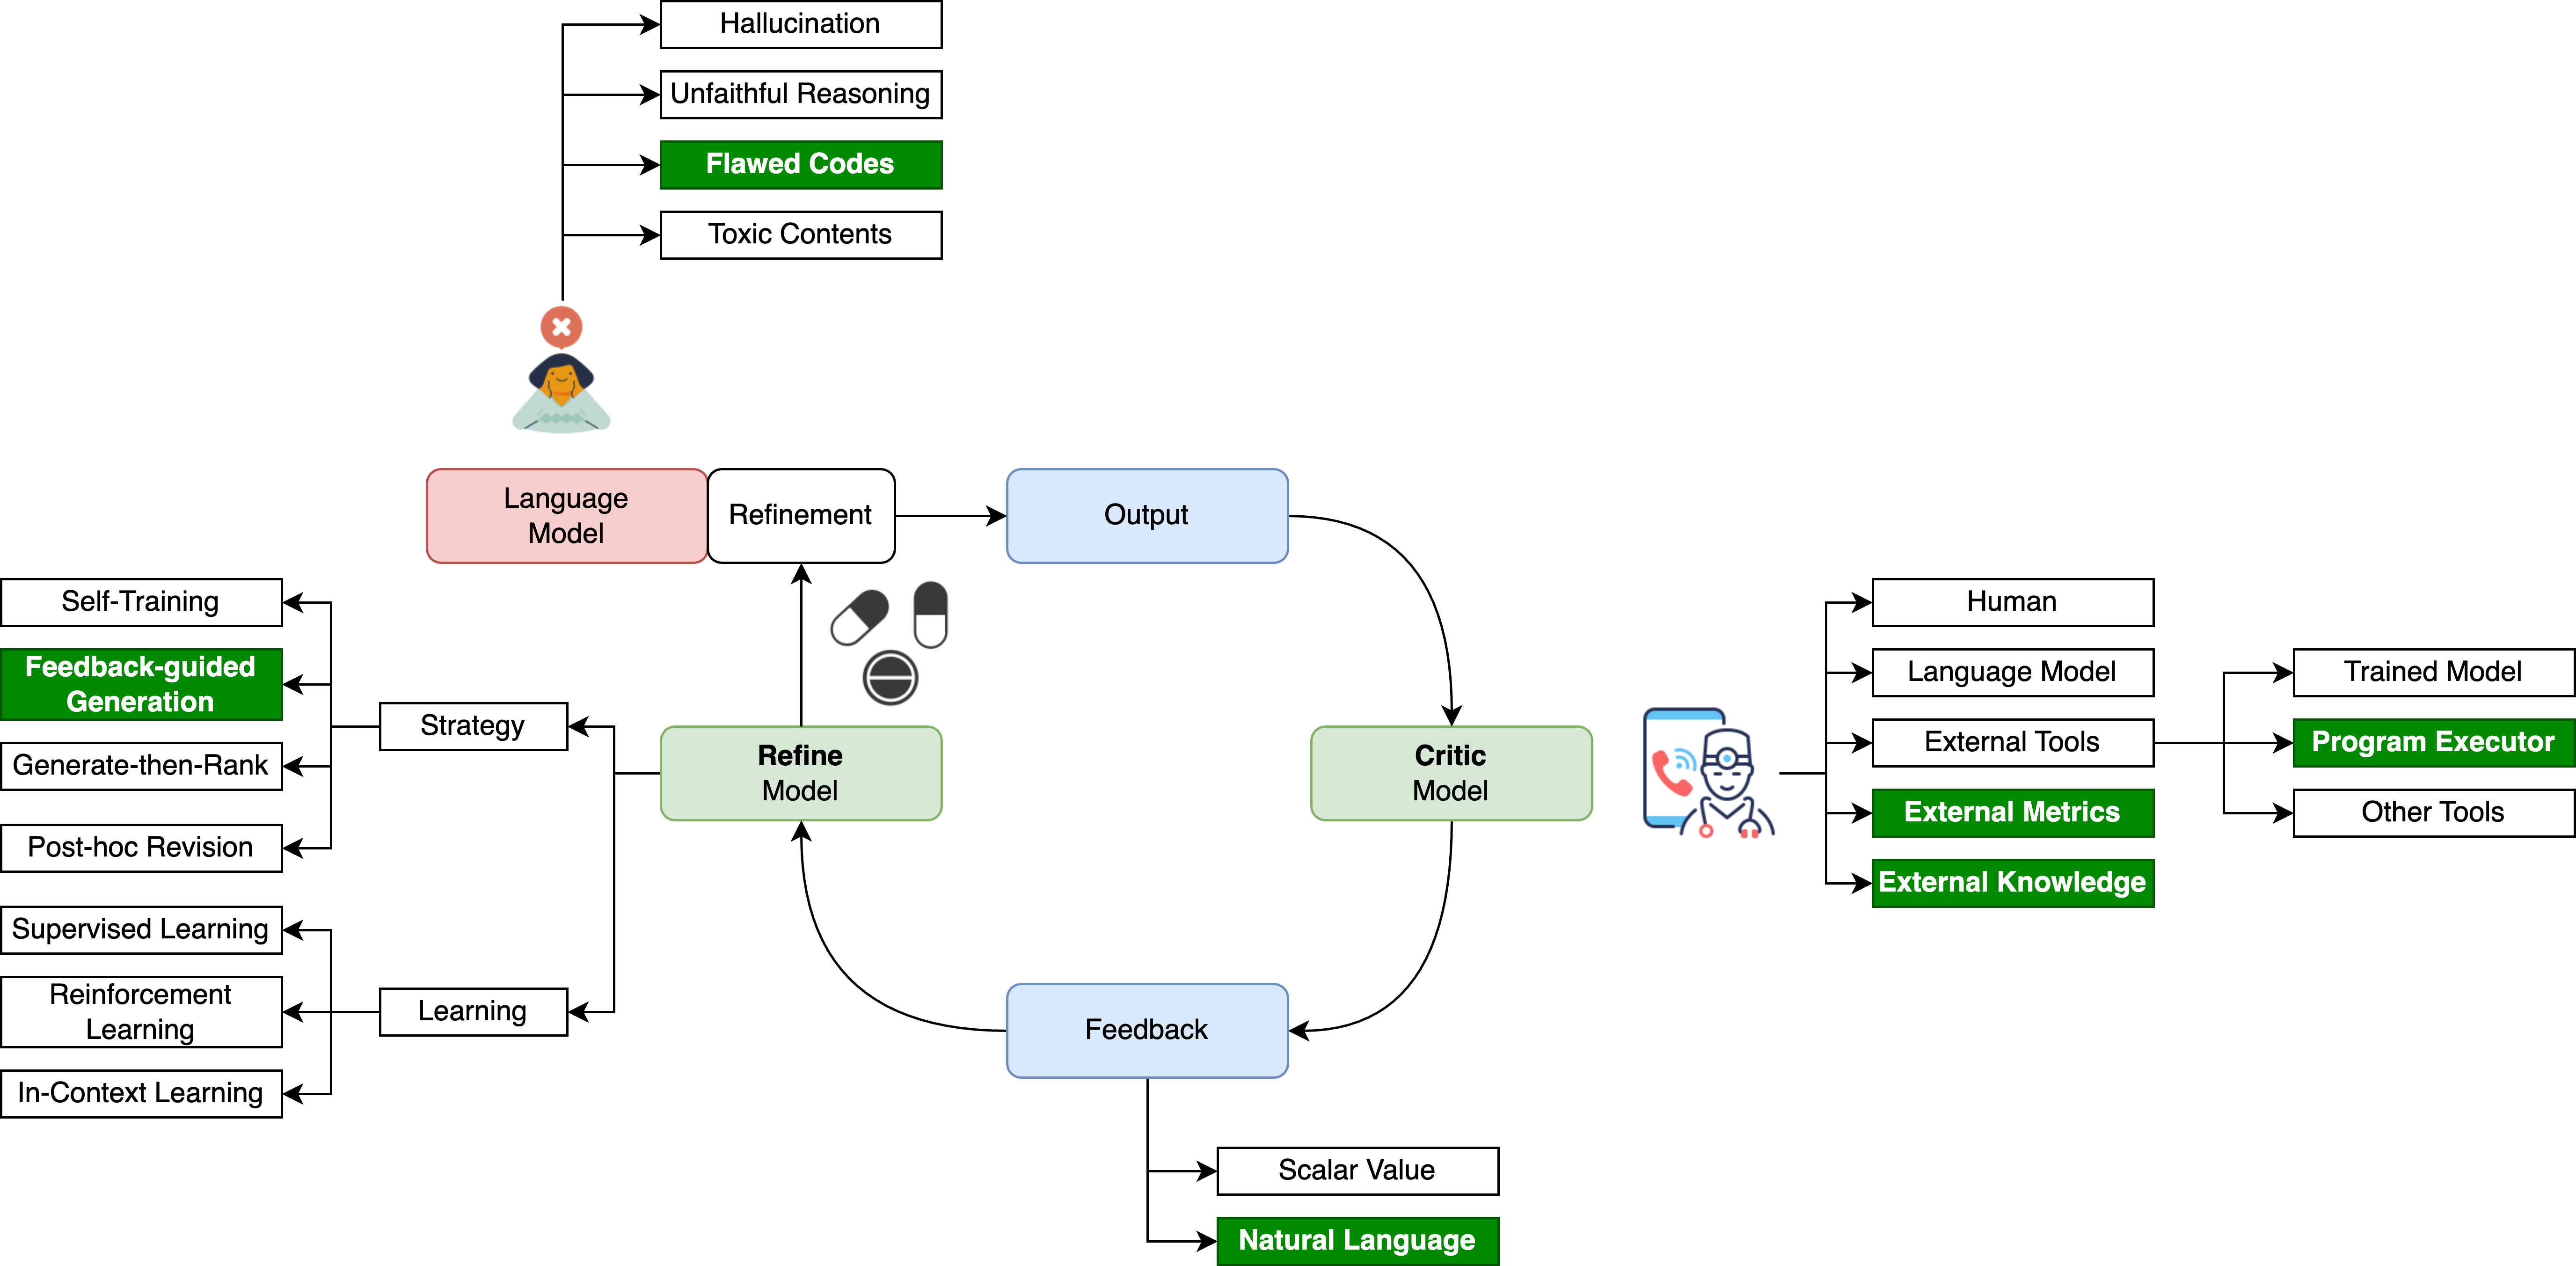
\includegraphics[width=1\textwidth]{img/direction_of_research}
        \captionsetup{font=small,labelformat=empty}
        \caption{Research Direction.}
    \end{figure}
\end{frame}
